\section{Apply the privacy-by-design principles using PE-BPMN}

We analysed our improved BPMN model (which is now GDPR compliant with added
annotations) and discovered several shortcomings---namely, the PSP and PLT can
put together the customer's identity and the location of their car, even when
this is not needed. For providing the parking service, it is sufficient if only
PLT learns of the parking location, and PSP of the user's identity. Moreover,
the PSP can read the parking permit information even though at this point the
PSP does not need to access these contents.

To help identify issues with the current process model, we used a tool called
Pleak \cite{pleaktool}. Pleak helps them to detect potential privacy risks by
identifying sensitive data, analysing data dependencies and performing
differentially private
computations~\cite[311-313]{10.1007/978-3-030-16722-6_18}. It also provides an
easy-to-use graphical interface for modellers to specify their business
processes and associated data flows~\cite{pleaktool}. The tool can quantify to
what extent a given output leaks information about the input, either in terms of
a sensitivity measure or in terms of the guessing advantage that an attacker
gains by having the output. Additionally, Pleak is a privacy-enhanced extension
of BPMN that enables the modelling of a wide variety of privacy-enhancing
technologies. This enables the analysis of privacy leakage risks and provides a
way to design processes that are more secure and compliant with privacy
regulations~\cite[1-3]{10.1007/s10009-021-00636-w}. Pleak is therefore a great
tool for helping to ensure compliance with data minimisation principles, such as
those outlined in the GDPR.

To protect the customer's data from parties not privy to certain details, we
opted for data encryption. The alternatives would have been secret sharing, data
splitting, or a hybrid approach. While the hybrid approach might offer some more
benefits in terms of privacy, using the encryption approach seemed to be the 
most rational in the current case, as there is no handling of any special type
of personal data (like health data, which might require higher levels of
protection). Adding third parties always comes with additional complexity, which
we did not wish to introduce here.

We note that our scheme assumes that a mechanism for key-exchange has been
agreed upon separately, and keys exchanged beforehand, for example during the
registration flow. The same assumption goes for the license plate information.
We did not add the key-exchange to the model as it is out of scope.

\newpage
The analysis of the model depicted on Figure~\ref{fig:improved-model} provided
the following results:

\begin{center}
\begin{tabular}{ |c||c|c|c|c|c|c|c|c|c|c|c|c|c| } 
    \hline
    & 1 & 2 & 3 & 4 & 5 & 6 & 7 & 8 & 9 & 10 & 11 & 12 & 13\\ 
    \hline
    \hline
    PLT [Processor] & V & - & - & - & V & - & - & V & - & V & V & - & -\\
    \hline
    PSP [Controller] & - & V & V & - & - & V & V & V & - & - & V & V & -\\
    \hline
    User device & - & - & - & O & - & - & - & V & V & - & - & O & -\\
    \hline
    \hline
    Shared over & - & - & - &
    \multicolumn{1}{m{1.2em}|}{MF (V)} &
    \multicolumn{1}{m{1.2em}|}{MF (V)} &
    \multicolumn{1}{m{1.2em}|}{MF (V)} &
    \multicolumn{1}{m{1.2em}|}{MF (V)} &
    \multicolumn{1}{m{1.2em}|}{MF (V)} &
    - & - &
    \multicolumn{1}{m{1.2em}|}{MF (V)} &
    \multicolumn{1}{m{1.2em}|}{MF (V)} & -\\
    \hline
\end{tabular}
\\~\\
V = visible, H = hidden, O = owner, MF = MessageFlow, S = SecureChannel
\end{center}
where the header row numbers represent the following:
\begin{enumerate}
    \item PLTParkingPermitStorage
    \item {[Artifact]} Consent
    \item {[Artifact]} RecordOfProcessing
    \item {[personal\_data]} location
    \item availabilityNotification
    \item location
    \item loginNotification
    \item parkingPermit (PLT name, parking spot, vehicle plate)
    \item parkingPermitStorage
    \item parkingRequest (location)
    \item parkingReservation (location, vehicle plate)
    \item parkingServiceCredential
    \item {[Artifact]} PrivacyPolicy
\end{enumerate}

The results clearly show that the PSP can access the location of the user and
the parking permit, while PSP does not require access to those details. Using
encryption, we complemented our model by utilizing encryption and secure
communication channels. The complemented model is shown on
Figure~\ref{fig:pleak-model}.

\begin{landscape}

\begin{figure}[ht]
\begin{center}
    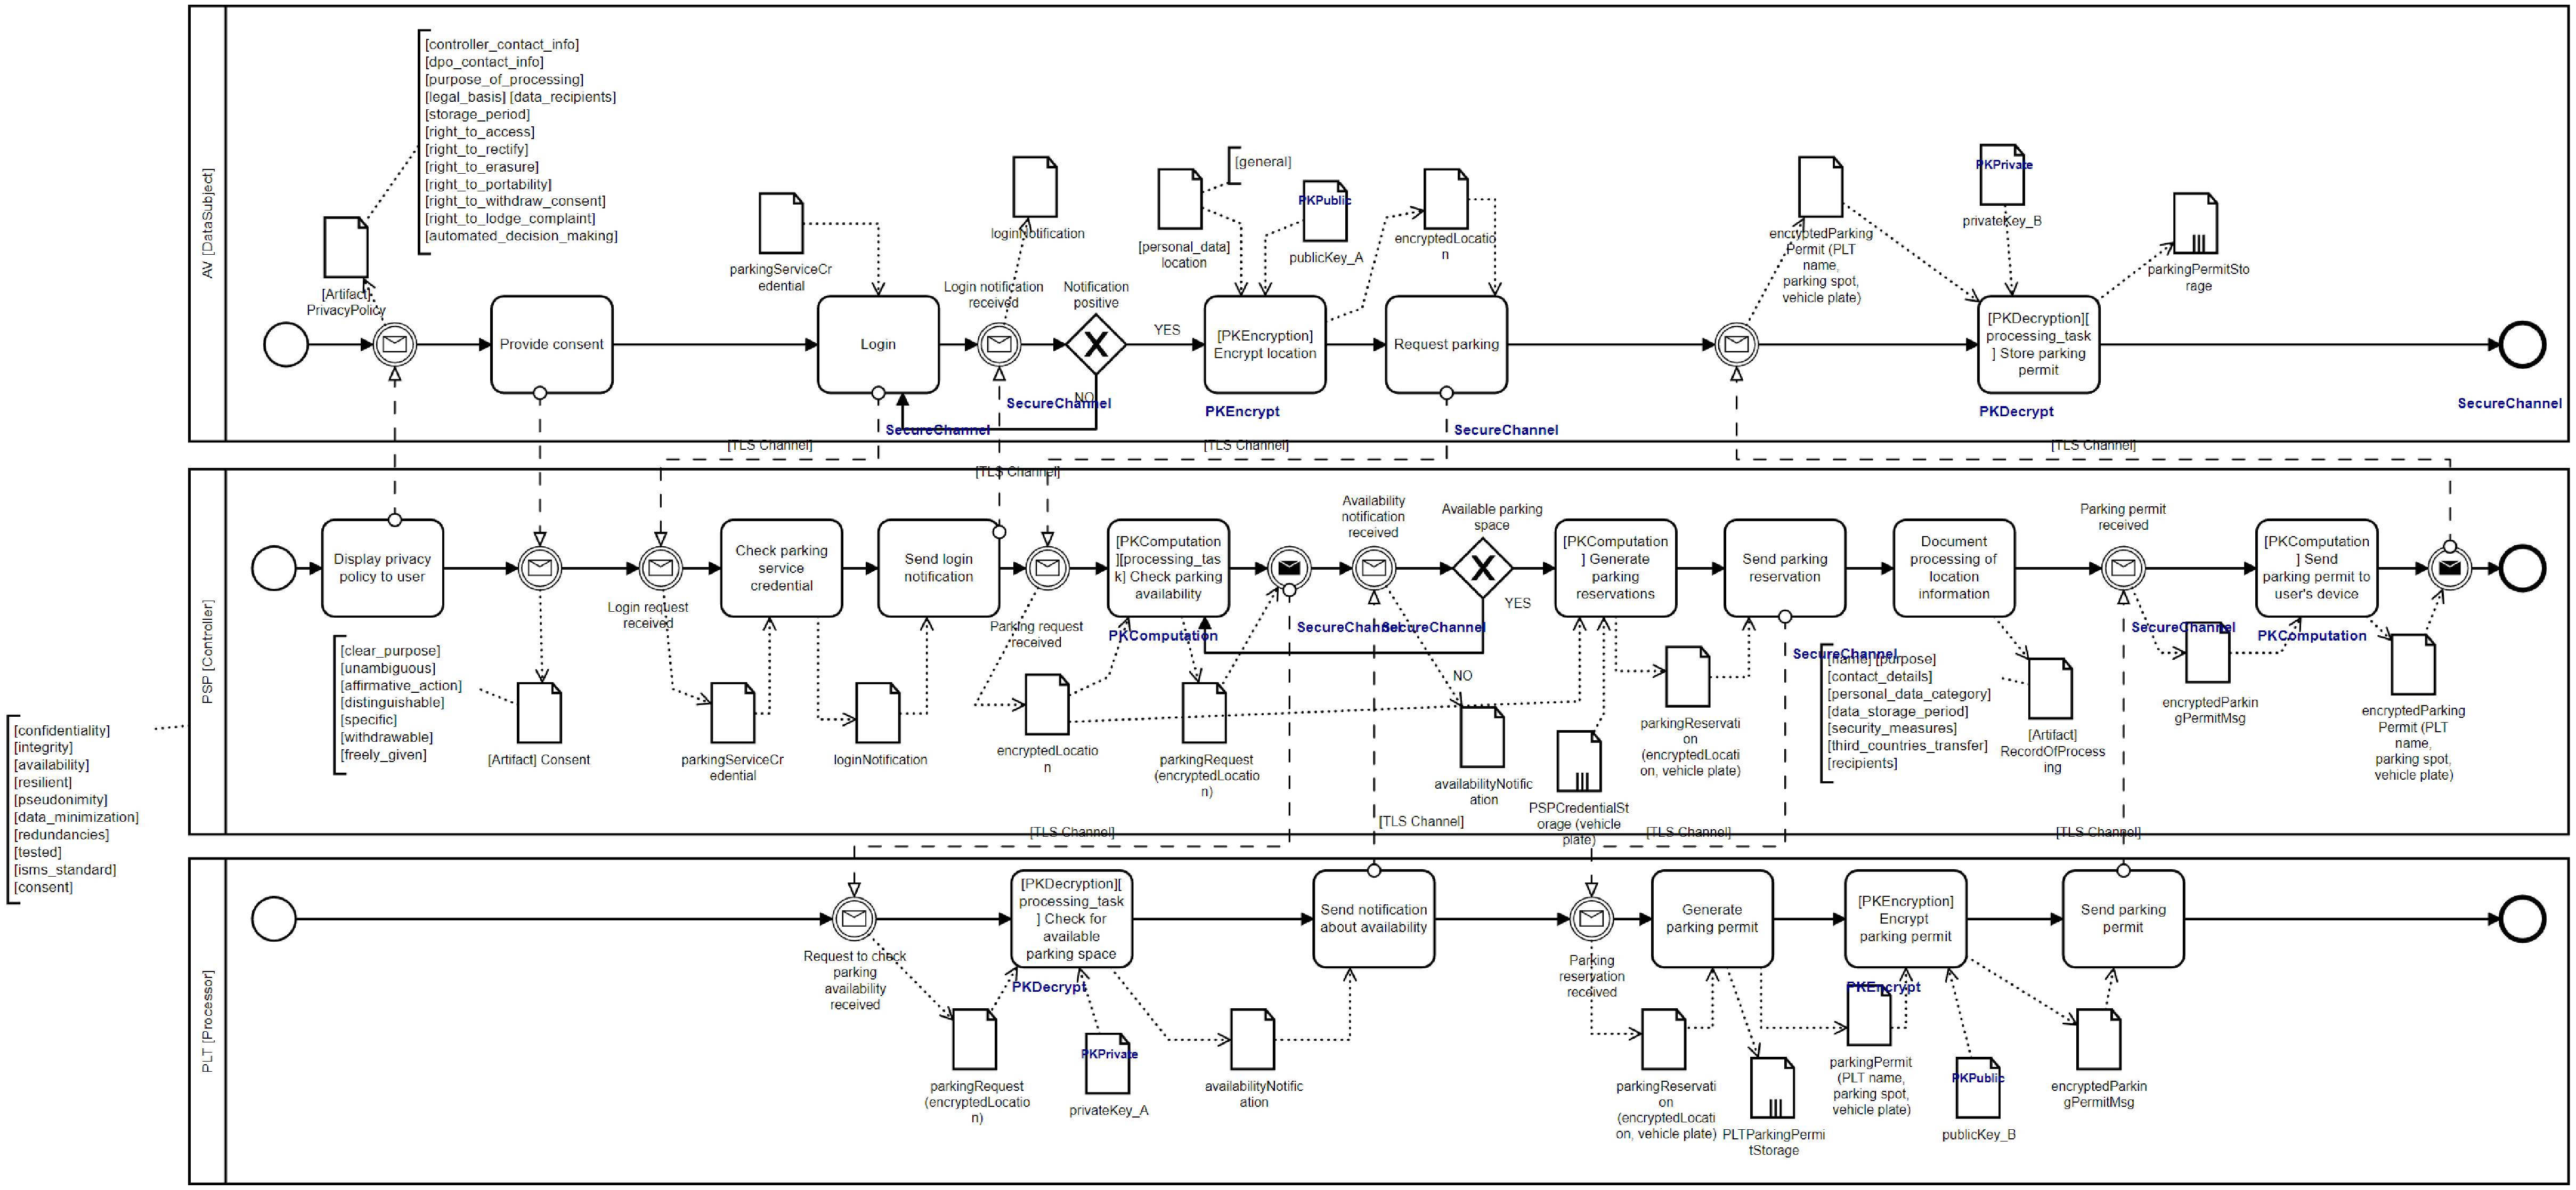
\includegraphics[height=\textwidth - 136pt]{pleak.pdf}
    \caption{PE-BPMN model}
    \label{fig:pleak-model}
\end{center}
\end{figure}

\end{landscape}

The analysis of our complemented model yields the following results:

\vspace{1em} % newline hack
\centerline{
\begin{tabular}{ |c||c|c|c|c|c|c|c|c|c|c|c|c|c|c|c|c| } 
    \hline
    & 1 & 2 & 3 & 4 & 5 & 6 & 7 & 8 & 9 & 10 & 11 & 12 & 13 & 14 & 15 & 16\\ 
    \hline
    \hline
    AV [DataSubject] & - & - & - & V & - & O & V & - & V & - & - & O & - & O &
    O & -\\
    \hline
    PLT [Processor] & V & - & - & - & - & - & - & V & - & V & V & - & O & - &
    - & O\\
    \hline
    PSP [Controller] & - & O & V & - & V & H & V & H & H & V & V & V & - & - &
    - & -\\
    \hline
    \hline
    Shared over & - & - & - & - & - & S & S & S & S & S & S & S & - & - & - &
    -\\
    \hline
\end{tabular}
}
\begin{center}
V = visible, H = hidden, O = owner, MF = MessageFlow, S = SecureChannel
\end{center}
where the header row numbers represent the following:
\begin{enumerate}
    \item PLTParkingPermitStorage
    \item PSPCredentialStorage (vehicle plate)
    \item {[Artifact]} Consent
    \item {[Artifact]} PrivacyPolicy
    \item {[Artifact]} RecordOfProcessing
    \item {[personal\_data]} location, encryptedLocation
    \item loginNotification
    \item encryptedParkingPermitMsg, parkingPermit(PLT name, parking spot,
    vehicle plate)
    \item encryptedParkingPermit (PLT name, parking spot, vehicle plate),
    parkingPermitStorage
    \item availabilityNotification, parkingRequest (encryptedLocation)
    \item parkingReservation (encryptedLocation, vehicle plate)
    \item parkingServiceCredential
    \item privateKey\_A
    \item privateKey\_B
    \item publicKey\_A
    \item publicKey\_B
\end{enumerate}
